\chapter{المواد النقية والخلائط}\label{ch:g6:pure-substances-and-mixtures}

تذكر قارورة الماء المعدني على ملصقها نحو اثنتي عشرة مادة ذائبة، مع
مقاديرها بالمليغرام في اللتر. أما الماء الذي يخرج من جهاز التنقية في
المختبر فلا تُذكر له أي مادة. كلاهما رائق عديم اللون، وكلاهما يروي
العطش --- لكن واحدًا منهما فقط هو ما يسميه الكيميائي نقيًّا. يعطي هذا الفصل
كلمة «نقي» معناها الدقيق، ويبيّن كيف نميّز \omterm{def:g6:pure-substances-and-mixtures:pure-substance}{المادة النقية} من \omterm{def:g6:pure-substances-and-mixtures:mixture}{الخليط}
دون أن نتذوق شيئًا.

\begin{recall}
\omterm{def:g2:mixing-and-dissolving:mix}{الخلط} أن نضع أشياء مختلفة معًا؛ والجسم الصلب الذي \omterm{def:g2:mixing-and-dissolving:dissolve}{يذوب} في الماء يترك
السائل رائقًا، والسائل الرائق \omterm{def:g2:mixing-and-dissolving:dissolve}{محلول}
(\cref{ch:g2:mixing-and-dissolving}). ويمكن فصل مكونات الخلائط
\omterm{def:g3:separating-mixtures:sieve}{بالغربلة} \omterm{def:g3:separating-mixtures:decant}{والترويق} \omterm{def:g3:separating-mixtures:filter}{والترشيح} \omterm{def:g3:separating-mixtures:evaporate}{والتبخير}
(\cref{ch:g3:separating-mixtures}). ولكل مادة خصائص يمكن اختبارها:
صلبة أو لينة، شفافة أو غير شفافة، تطفو أو تغوص
(\cref{ch:g1:materials-around-us}).
\end{recall}

\section{الأنواع الكيميائية والمواد النقية}

\begin{definition}[النوع الكيميائي]\label{def:g6:pure-substances-and-mixtures:species}
\emph{النوع الكيميائي}\index{نوع كيميائي} صنف معيّن من المواد، له اسمه
الخاص وخصائصه الخاصة: الماء، والسكر، والملح، والأكسجين، والإيثانول
(كحول النبيذ)، والحديد.
\end{definition}

\begin{definition}[المادة النقية]\label{def:g6:pure-substances-and-mixtures:pure-substance}
\emph{المادة النقية}\index{مادة نقية} مادة مكوّنة من \omterm{def:g6:pure-substances-and-mixtures:species}{نوع كيميائي} واحد
لا غير: الماء المقطر، وبلورة السكر، وخاتم من الذهب الخالص.
\end{definition}

\begin{definition}[الخليط]\label{def:g6:pure-substances-and-mixtures:mixture}
\emph{الخليط}\index{خليط} يحوي عدة أنواع كيميائية. \omterm{def:g4:air-a-mixture-of-gases:air}{فالهواء}، وماء البحر،
والماء المعدني، والحليب، والغرانيت، وعصير البرتقال خلائط.
\end{definition}

\begin{remark}[النقي في اللغة اليومية]\label{rem:g6:pure-substances-and-mixtures:everyday}
عبارة «عصير برتقال نقي» على العلبة تعني أنه لم يُضف شيء إلى العصير.
أما عند الكيميائي فالعصير يبقى خليطًا: ماء، وسكريات، وأحماض، وفيتامينات،
وملوّنات، ونكهات، أي أنواع كيميائية كثيرة. و«ماء الجبال النقي» \omterm{def:g6:pure-substances-and-mixtures:mixture}{خليط}
أيضًا: ماء فيه أملاح ذائبة.
\end{remark}

\begin{omfigure}
\begin{tikzpicture}[font=\small, level distance=1.55cm,
    box/.style={draw=omDef, fill=omDef!6, rounded corners=2pt, align=center,
      inner sep=4pt},
    level 1/.style={sibling distance=7.2cm},
    level 2/.style={sibling distance=3.6cm},
    edge from parent/.style={draw, thick, omDef, ->}]
  \node[box] {المادة}
    child {node[box] {مادة نقية\\ \footnotesize نوع كيميائي واحد}
      child {node[box, draw=black!40, fill=white] {ماء مقطر،\\ ملح، حديد}}}
    child {node[box] {خليط\\ \footnotesize عدة أنواع كيميائية}
      child {node[box] {متجانس\\ \footnotesize مظهر واحد في كل مكان}
        child {node[box, draw=black!40, fill=white] {ماء مالح،\\ هواء}}}
      child {node[box] {غير متجانس\\ \footnotesize أجزاؤه تُرى}
        child {node[box, draw=black!40, fill=white] {ماء موحل،\\ غرانيت}}}};
\end{tikzpicture}

{\small فرز المادة. الصناديق السفلى تعطي أمثلة على كل صنف.}
\end{omfigure}

\section{الخلائط المتجانسة وغير المتجانسة}

\begin{definition}[الخليط المتجانس والخليط غير المتجانس]\label{def:g6:pure-substances-and-mixtures:homogeneous}
يكون \omterm{def:g6:pure-substances-and-mixtures:mixture}{الخليط} \emph{خليطًا متجانسًا}\index{خليط متجانس} إذا تعذّر على
العين أن تميّز أجزاءه المختلفة، حتى بالعدسة المكبرة: فمظهره واحد في كل
مكان. ويكون \emph{خليطًا غير متجانس}\index{خليط غير متجانس} إذا أمكن
رؤية جزأين مختلفين منه على الأقل.
\end{definition}

\begin{example}[أربعة خلائط]\label{ex:g6:pure-substances-and-mixtures:four}
الماء المالح \omterm{def:g4:air-a-mixture-of-gases:air}{والهواء} متجانسان: أجزاؤهما لا تُرى. والزيت فوق الماء غير
متجانس: طبقتان. والماء الموحل غير متجانس: تسبح فيه حبيبات ثم تترسب.
وعصير البرتقال باللب غير متجانس: قطع اللب تُرى.
\end{example}

\begin{omfigure}
\begin{tikzpicture}[font=\small, scale=1.15]
  \pic[transform shape] at (0,0) {beaker={0.7}{omWater!80}};
  \node[anchor=north, align=center] at (0,-0.15) {ماء مالح:\\ متجانس};
  \pic[transform shape] at (2.6,0) {beaker={0.7}{omWater!80}};
  \fill[yellow!55!orange!60] (1.8,1.05) rectangle (3.4,1.4);
  \draw[omGlass, line width=0.7pt] (1.8,1.05) -- (1.8,1.4) (3.4,1.05) -- (3.4,1.4);
  \node[anchor=north, align=center] at (2.6,-0.15) {زيت فوق ماء:\\ غير متجانس};
  \pic[transform shape] at (5.2,0) {beaker={0.7}{brown!25}};
  \foreach \x/\y in {4.6/0.3,4.9/0.7,5.3/0.5,5.6/1.0,5.0/1.1,5.4/0.2,5.8/0.6}
    \fill[brown!65] (\x,\y) circle (0.04);
  \fill[brown!60] (4.4,0) rectangle (6.0,0.12);
  \node[anchor=north, align=center] at (5.2,-0.15) {ماء موحل:\\ غير متجانس};
  \pic[transform shape] at (7.8,0) {beaker={0.7}{orange!45}};
  \foreach \x/\y in {7.3/0.35,7.6/0.8,8.0/0.5,8.3/1.0,7.7/1.15,8.2/0.25,7.45/0.65}
    \fill[orange!80!brown] (\x,\y) ellipse (0.08 and 0.03);
  \node[anchor=north, align=center] at (7.8,-0.15) {عصير باللب:\\ غير متجانس};
\end{tikzpicture}

{\small \omterm{def:g6:pure-substances-and-mixtures:homogeneous}{خليط متجانس} واحد وثلاثة خلائط غير متجانسة.}
\end{omfigure}

\begin{omfigure}
\begin{minipage}[b]{0.48\linewidth}\centering
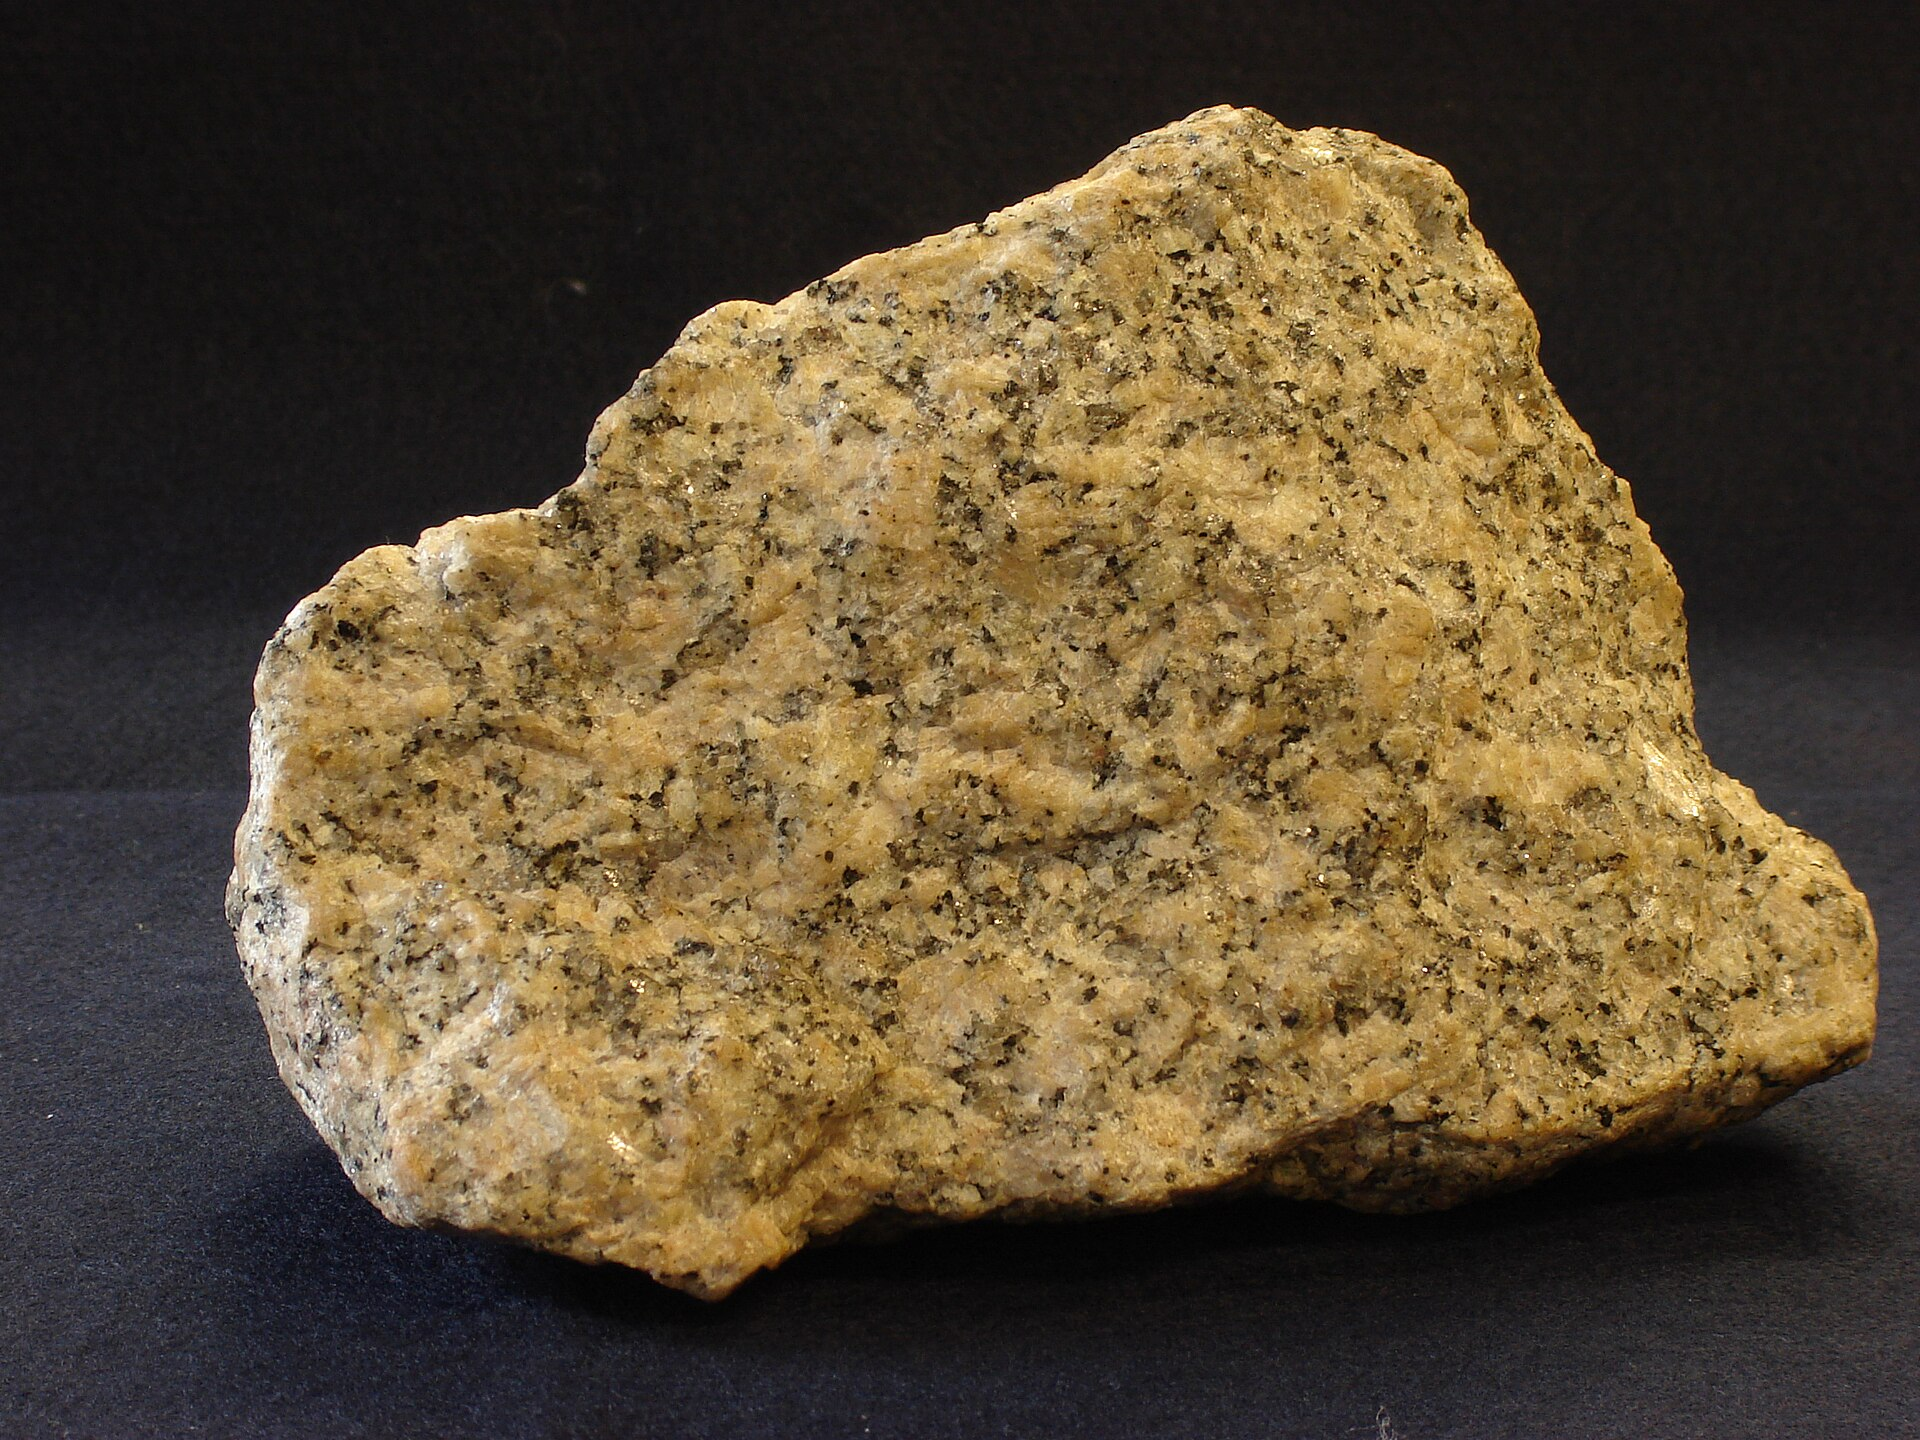
\includegraphics[width=\linewidth,height=4.6cm,keepaspectratio]{images/book1/granite.jpg}

{\small الغرانيت: تُرى فيه حبيبات من ثلاثة معادن أو أربعة مختلفة.
جسم صلب غير متجانس. تصوير: يوريكو زيمبريس، CC BY-SA 2.0 br.}
\end{minipage}\hfill
\begin{minipage}[b]{0.48\linewidth}\centering
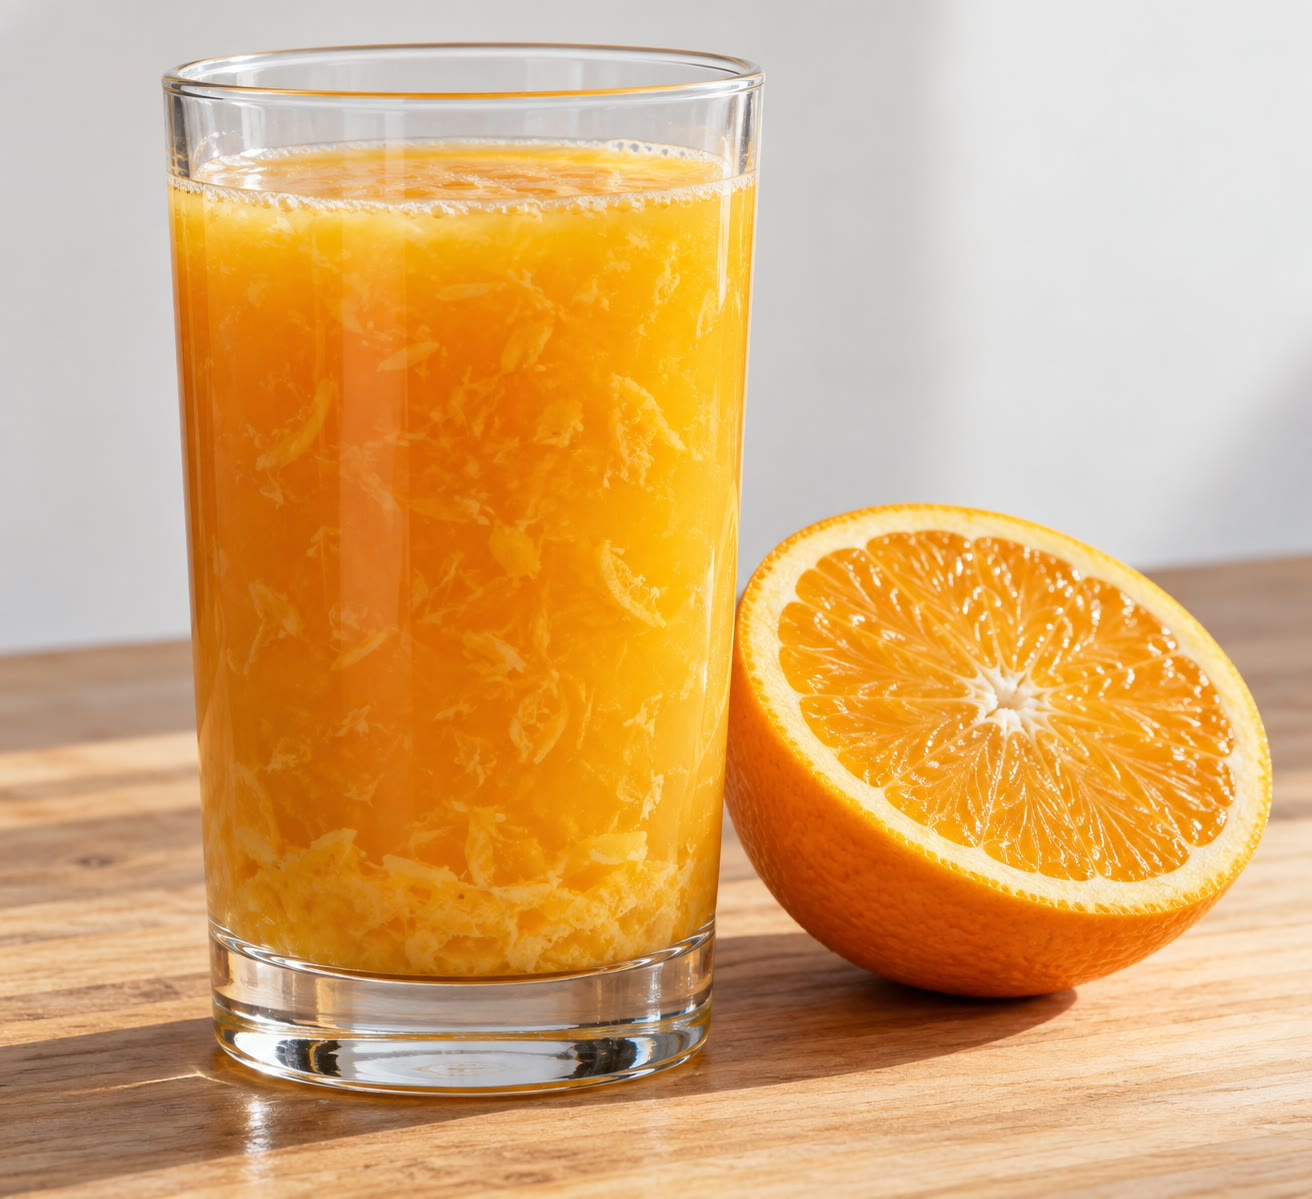
\includegraphics[width=\linewidth,height=4.6cm,keepaspectratio]{images/book1/ai/g6-orange-juice.jpg}

{\small عصير برتقال باللب: \omterm{def:g6:pure-substances-and-mixtures:homogeneous}{خليط غير متجانس}.}
\end{minipage}
\end{omfigure}

\begin{remark}[المتجانس لا يعني النقي]\label{rem:g6:pure-substances-and-mixtures:not-pure}
الماء المالح يشبه الماء النقي تمامًا. فالنظر لا يكفي لتمييز \omterm{def:g6:pure-substances-and-mixtures:pure-substance}{المادة
النقية} من \omterm{def:g6:pure-substances-and-mixtures:homogeneous}{الخليط المتجانس}: لا بد أن نقيس شيئًا.
\end{remark}

\section{التعرف على المادة النقية بثوابتها}

\begin{proposition}[للمادة النقية ثوابتها الخاصة]\label{prop:g6:pure-substances-and-mixtures:constants}
% ledger: mp:water, bp:water, bp:ethanol, mp:ethanol, rho:water, rho:ethanol, mp:NaCl, mp:Fe, rho:Fe
كل \omterm{def:g6:pure-substances-and-mixtures:pure-substance}{مادة نقية} تنصهر عند درجة حرارة ثابتة خاصة بها، وتغلي عند درجة حرارة
ثابتة خاصة بها (تحت الضغط العادي)، ولها كتلة خاصة بها لحجم معيّن، هي
كثافتها. هذه الأعداد هي ثوابتها؛ ويشرح كتاب الفيزياء ما تقيسه. وهذه
ثوابت بعض المواد النقية:
\begin{center}
\small
\begin{tabular}{lccc}
\hline
\omterm{def:g6:pure-substances-and-mixtures:pure-substance}{المادة النقية} & تنصهر عند & تغلي عند & كتلة \qty{1}{cm^3} \\
\hline
الماء & \qty{0}{\celsius} & \qty{100}{\celsius} & نحو \qty{1.0}{g} \\
الإيثانول & \qty{-114}{\celsius} & \qty{78}{\celsius} & \qty{0.79}{g} \\
البروبانون (الأسيتون) & --- & \qty{56}{\celsius} & \qty{0.78}{g} \\
الملح (كلوريد الصوديوم) & \qty{801}{\celsius} & --- & \qty{2.17}{g} \\
الحديد & \qty{1538}{\celsius} & --- & \qty{7.87}{g} \\
\hline
\end{tabular}
\end{center}
% ledger: bp:acetone, rho:acetone, rho:NaCl
\end{proposition}

\begin{proposition}[الخليط ليس له درجة غليان ثابتة]\label{prop:g6:pure-substances-and-mixtures:mixture-boils}
\omterm{def:g6:pure-substances-and-mixtures:mixture}{الخليط} لا يغلي عند درجة حرارة واحدة ثابتة: فالماء المالح يبدأ في الغليان
فوق \qty{100}{\celsius} بقليل، وتواصل درجة حرارته الارتفاع في أثناء
الغليان، إذ يذهب الماء ويزداد تركيز الملح الذي يبقى.
\end{proposition}

\begin{method}[هل هذا السائل نقي؟ وما هو؟]\label{met:g6:pure-substances-and-mixtures:identify}
\begin{enumerate}
  \item سخّنه في المختبر، واقرأ درجة حرارته في أثناء
        غليانه.
  \item إذا بقيت درجة الحرارة ثابتة فالسائل على الأرجح \omterm{def:g6:pure-substances-and-mixtures:pure-substance}{مادة نقية}:
        قارن تلك الدرجة بجدول للثوابت.
  \item إذا واصلت درجة الحرارة الارتفاع فهو \omterm{def:g6:pure-substances-and-mixtures:mixture}{خليط}.
  \item تحقق بثابت ثانٍ، مثل كتلة حجم
        معلوم.
\end{enumerate}
\end{method}

\begin{inthelab}[غليان الماء المالح]
يسخّن المعلم ماءً نقيًا وماءً مالحًا جنبًا إلى جنب، وفي كل منهما مقياس
حرارة. يغلي الماء النقي عند \qty{100}{\celsius} ويبقى عندها ما دام يغلي.
أما الماء المالح فيبدأ في الغليان فوق \qty{100}{\celsius} بقليل، ويزحف
مقياس الحرارة صعودًا دقيقة بعد دقيقة.
\end{inthelab}

\section{الماء، النقي وغير النقي}

\begin{example}[أربعة أنواع من الماء]\label{ex:g6:pure-substances-and-mixtures:waters}
% ledger: sea:salinity
\begin{itemize}
  \item \textbf{الماء المقطر}، الذي يُحضَّر في المختبر، يكاد يكون \omterm{def:g6:pure-substances-and-mixtures:pure-substance}{مادة
        نقية}: ماء لا غير.
  \item \textbf{ماء الصنبور} \omterm{def:g6:pure-substances-and-mixtures:homogeneous}{خليط متجانس}: ماء فيه مقادير صغيرة من مواد
        ذائبة (القطرة التي تجف على صحن داكن تترك حلقة
        بيضاء).
  \item \textbf{الماء المعدني} \omterm{def:g6:pure-substances-and-mixtures:homogeneous}{خليط متجانس} يذكر ملصقه المواد الذائبة،
        بالمليغرام في اللتر.
  \item \textbf{ماء البحر} \omterm{def:g6:pure-substances-and-mixtures:homogeneous}{خليط متجانس} يحوي نحو
        \qty{35}{g} من الأملاح في كل كيلوغرام.
\end{itemize}
\end{example}

\begin{omfigure}
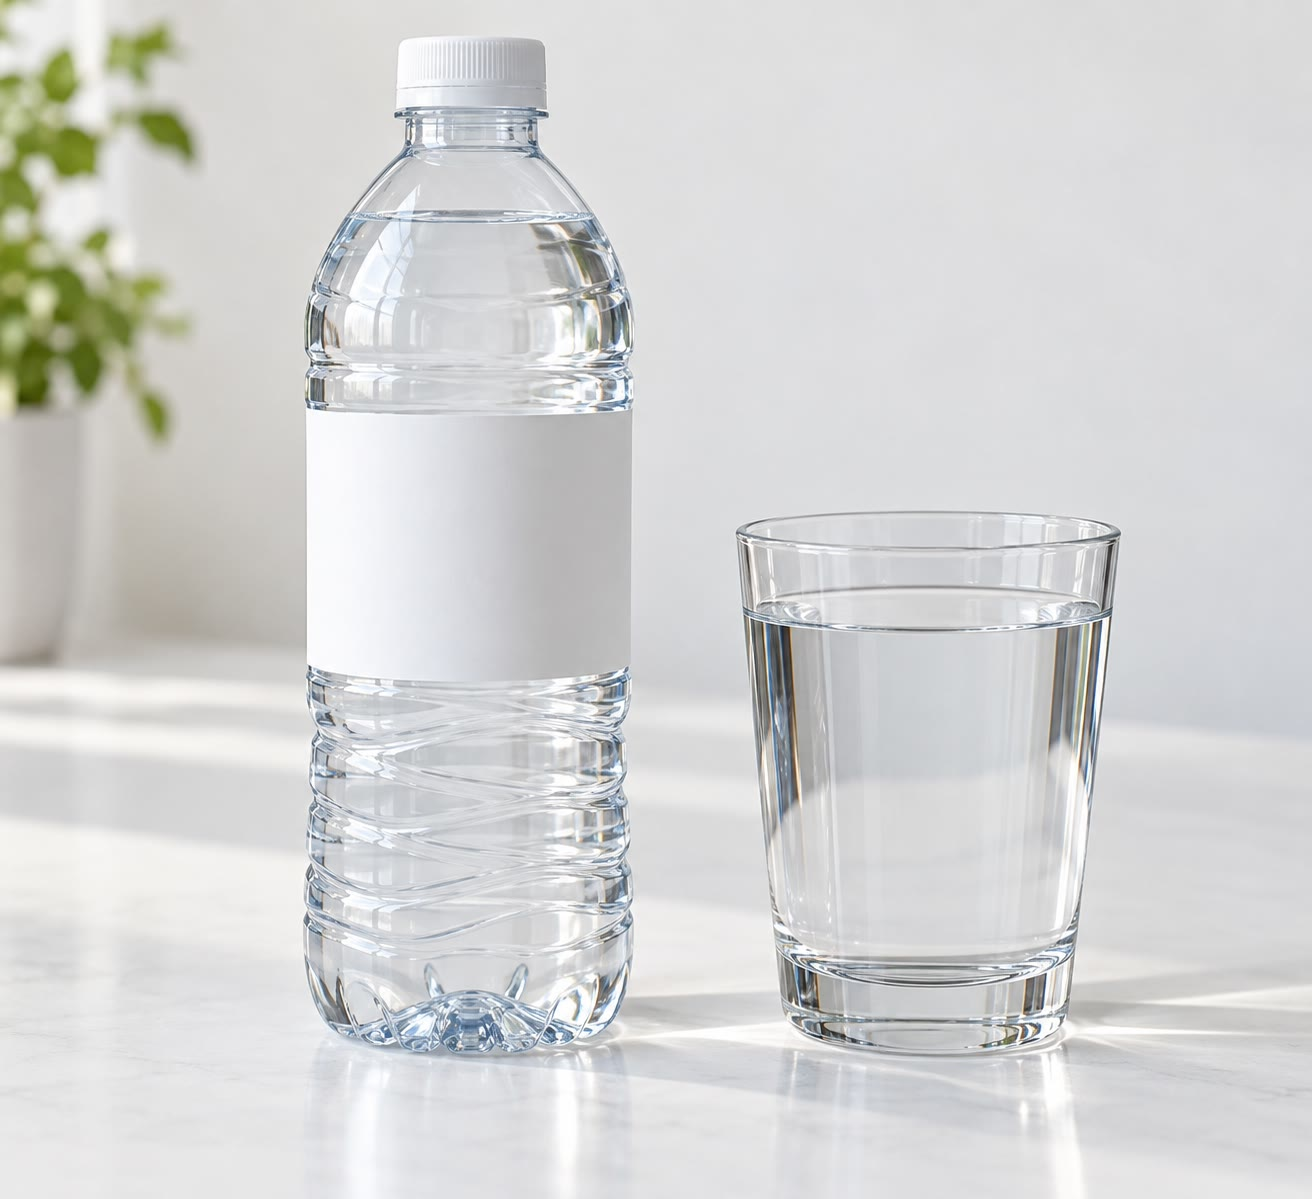
\includegraphics[width=0.5\linewidth]{images/book1/ai/g6-mineral-water.jpg}

{\small قارورة ماء معدني: رائق عديم اللون، ومع ذلك فهو
\omterm{def:g6:pure-substances-and-mixtures:mixture}{خليط}.}
\end{omfigure}

\begin{example}[قراءة ملصق الماء المعدني]\label{ex:g6:pure-substances-and-mixtures:label}
يقول ملصق: الكالسيوم \qty{78}{mg/L}، والمغنيسيوم \qty{24}{mg/L}،
والصوديوم \qty{5}{mg/L}، وهيدروجين الكربونات \qty{357}{mg/L}، والكبريتات
\qty{10}{mg/L}، والكلوريد \qty{4}{mg/L}. (هذه الأرقام مثال.)
ففي لتر واحد $78 + 24 + 5 + 357 + 10 + 4 = 478$\,mg من
المواد الذائبة، أي نحو نصف غرام: مقدار ضئيل إلى جانب \qty{1000}{g}
من الماء، لكنه يكفي لجعله خليطًا.
\end{example}

\section{تمارين}

\begin{exercise}[$\star$]\label{exo:g6:pure-substances-and-mixtures:1}
\omterm{def:g6:pure-substances-and-mixtures:pure-substance}{مادة نقية} أم \omterm{def:g6:pure-substances-and-mixtures:mixture}{خليط}؟ الماء المقطر، \omterm{def:g4:air-a-mixture-of-gases:air}{والهواء}، وماء البحر، وكتلة من الحديد
الخالص، والحليب، وبلورة سكر.
\end{exercise}

\begin{exercise}[$\star$]\label{exo:g6:pure-substances-and-mixtures:2}
متجانس أم غير متجانس؟ الماء المالح، والغرانيت، والزيت فوق الماء، وماء
الصنبور، والموسلي.
\end{exercise}

\begin{exercise}[$\star$]\label{exo:g6:pure-substances-and-mixtures:3}
ما \omterm{def:g6:pure-substances-and-mixtures:species}{النوع الكيميائي}؟ أعطِ ثلاثة أمثلة.
\end{exercise}

\begin{exercise}[$\star$]\label{exo:g6:pure-substances-and-mixtures:4}
يغلي سائل عند \qty{78}{\celsius}، وتبقى درجة حرارته عند
\qty{78}{\celsius} في أثناء غليانه. استعن بجدول الثوابت لتقترح
ما هو.
\end{exercise}

\begin{exercise}[$\star$]\label{exo:g6:pure-substances-and-mixtures:5}
لماذا لا يُعدّ «عصير البرتقال النقي» \omterm{def:g6:pure-substances-and-mixtures:pure-substance}{مادة نقية} عند الكيميائي؟
\end{exercise}

\begin{exercise}[$\star\star$]\label{exo:g6:pure-substances-and-mixtures:6}
يبدأ سائل في الغليان عند \qty{100.5}{\celsius} وترتفع درجة حرارته في أثناء
غليانه. هل هو \omterm{def:g6:pure-substances-and-mixtures:pure-substance}{مادة نقية}؟ وماذا يمكن أن يكون؟
\end{exercise}

\begin{exercise}[$\star\star$]\label{exo:g6:pure-substances-and-mixtures:7}
انظر إلى شكل الكؤوس الأربع. في أي كأس يمكن لمرشِّح أن يفصل أجزاء
\omterm{def:g6:pure-substances-and-mixtures:mixture}{الخليط}؟ وفي أي كأس لا يمكنه؟
\end{exercise}

\begin{exercise}[$\star\star$]\label{exo:g6:pure-substances-and-mixtures:8}
مكعب فلزي حجمه \qty{10}{cm^3} وكتلته \qty{78.7}{g}. ما كتلة
\qty{1}{cm^3}؟ وأي فلز من فلزات الجدول يمكن أن يكون؟
\end{exercise}

\begin{exercise}[$\star\star$]\label{exo:g6:pure-substances-and-mixtures:9}
مستعينًا بملصق الماء المعدني في المثال، ما النسبة المئوية من الكتلة الذائبة
التي يمثلها هيدروجين الكربونات؟ قرّب إلى أقرب عدد صحيح.
\end{exercise}

\begin{exercise}[$\star\star$]\label{exo:g6:pure-substances-and-mixtures:10}
يحوي ماء البحر نحو \qty{35}{g} من الأملاح في الكيلوغرام. ما كتلة
الأملاح في دلو من ماء البحر كتلته \qty{2}{kg}؟ وما النسبة المئوية للملح من
كتلة ماء البحر؟
\end{exercise}

\begin{exercise}[$\star\star\star$]\label{exo:g6:pure-substances-and-mixtures:11}
سائلان رائقان عديما اللون متطابقان في المظهر. صف قياسين يُجريان في
المختبر يبيّنان هل هما \omterm{def:g6:pure-substances-and-mixtures:pure-substance}{المادة النقية}
نفسها.
\end{exercise}

\begin{exercise}[$\star\star\star$]\label{exo:g6:pure-substances-and-mixtures:12}
\omterm{def:g6:pure-substances-and-mixtures:mixture}{خليط} مكوّن من \qty{90}{g} من الماء و\qty{10}{g} من الإيثانول.
ما النسبة المئوية للإيثانول من كتلته؟ وهل يمكن التعرف عليه بجدول
الثوابت؟ علّل.
\end{exercise}

\section{مسألة: ثلاثة سوائل عديمة اللون}

\begin{problem}[{مسألة نهاية الأسبوع --- ثلاث قوارير بلا ملصقات فيها سائل رائق
عديم اللون، والقياسات التي تميّز بينها}]
\label{pb:g6:pure-substances-and-mixtures:1}
% ledger: bp:water, bp:ethanol, rho:water, rho:ethanol, rho:seawater, sea:salinity
يعثر مساعد مختبر على ثلاث قوارير، A وB وC، سقطت ملصقاتها. وفي كل
منها سائل رائق عديم اللون. والمختبر لا يستعمل إلا ثلاثة سوائل من هذا
النوع: الماء المقطر، والإيثانول، وماء بحر جُلب من رحلة ميدانية. فيُجري
المساعد ثلاثة أنواع من القياسات في المختبر.

\medskip
\noindent\textbf{الجزء الأول --- النظر.}
\begin{enumerate}
  \item السوائل الثلاثة متطابقة في المظهر تمامًا. هل يستطيع المساعد أن
        يعرف بالنظر أيها مواد نقية؟ علّل.
  \item إذا كان أحدها خليطًا، فهل هو متجانس أم غير متجانس؟
  \item أي نوع من القياسات يمكن أن يبيّن أن السائل \omterm{def:g6:pure-substances-and-mixtures:pure-substance}{مادة
        نقية}؟
\end{enumerate}

\medskip
\noindent\textbf{الجزء الثاني --- القياس.}
يُسخَّن كل سائل حتى يغلي. يغلي السائل A عند
\qty{100}{\celsius} وتبقى درجة حرارته عندها. ويغلي السائل B عند
\qty{78}{\celsius} ويبقى عندها. ويبدأ السائل C في الغليان عند
\qty{100.6}{\celsius}، وتواصل درجة حرارته الارتفاع ببطء. ثم
يوزن \qty{50.0}{mL} من كل سائل: A \qty{49.8}{g}، وB
\qty{39.5}{g}، وC \qty{51.2}{g}.
\begin{enumerate}[resume]
  \item أي السوائل مواد نقية؟ وأيها \omterm{def:g6:pure-substances-and-mixtures:mixture}{خليط}؟
  \item مستعينًا بجدول الثوابت في هذا الفصل، سمِّ السائلين A
        وB.
  \item احسب كتلة \qty{1}{mL} (أي \qty{1}{cm^3}) من كل
        سائل.
  \item هل تتفق هذه الكتل مع جوابك عن السؤال 5؟
  \item لماذا تواصل درجة حرارة السائل C الارتفاع في أثناء غليانه؟
\end{enumerate}

\medskip
\noindent\textbf{الجزء الثالث --- ماذا في السائل C؟}
يُترك \qty{100}{mL} من السائل C يجف في صحن. وحين يذهب الماء كله
تبقى \qty{3.5}{g} من بلورات بيضاء.
\begin{enumerate}[resume]
  \item ماذا يبيّن هذا الراسب عن السائل C؟
  \item مستعينًا بكتلة \qty{1}{mL} من C التي وجدتها في السؤال 6، جد
        كتلة \qty{100}{mL} من C، ثم النسبة المئوية للملح من كتلته
        (بمنزلة عشرية واحدة).
  \item يحوي ماء البحر نحو \qty{35}{g} من الأملاح في كل كيلوغرام. ما
        النسبة المئوية لذلك؟ قارن بالسؤال 10.
  \item استنتج: كم غرامًا من الملح يحوي كل لتر من السائل C، وهل السائل C
        هو ماء البحر؟
\end{enumerate}
\end{problem}
